
\documentclass[12pt]{article}
\usepackage[hidelinks]{hyperref}
\usepackage{array}
\usepackage{booktabs}
\usepackage{cite}
\newcommand{\superscript}[1]{\ensuremath{^{\textrm{#1}}}}
\newcommand{\subscript}[1]{\ensuremath{_{\textrm{#1}}}}
\usepackage{graphicx}
\usepackage{mathptmx}

\bibliographystyle{abbrv}
\begin{document}

\title{Bag of Words Semantic Object Classification Based on RGBD Images}
\author{Adam Kosiorek}
\maketitle
e-mail: kosiorek.adam@gmail.com
Affiliation: Institute of Automation and Robotics, The Faculty of Mechatronics 
of Warsaw University of Technology \\
Supervisor: Prof. dr hab. Barbara Siemiątkowska \\
Defense date: 11.02.2014 \\
Keywords: bag-of-visual-words, object-classification, rgbd, point-cloud, datasets

\abstract{ 

This paper reviews a Bag of Words (BoW) semantic object classification framework 
based on RGBD data registered by the Microsoft Kinect. We describe a BoW 
processing pipeline (region detection, feature extraction and vector 
quantization) and evaluate the most popular algorithms in terms of object 
classification performance. Salient region detection is done by SIFT, ISS3D and 
Uniform Sampling. Description is performed by FPFH, PFH and PFHRGB. Vector 
quantization was carried out by KMeans.  All-vs-All-trained SVM with the RBF 
kernel was used as a classifier. We review available point cloud databases in 
terms of usability in scene classification studies. We achieved the accuracy of 
65.22\% on 8 categories of the Berkeley 3D Object Dataset and 62.3\% on a 10 
category dataset compiled by Zhang.

}

%%%%%%%%%%%%%%%%%%%%%%%%%
%	Po Polsku !!!
%%%%%%%%%%%%%%%%%%%%%%%%%%

\title{Semantyczna klasyfikacja obiektów na obrazach RGBD metodą Bag of Words}
Słowa kluczowe: bag-of-visual-words, object-classification, rgbd, chmura-punktów, zbiór-danych
\abstract{ 

W pracy przedstawiono metodę klasyfikacji metodą Bag of Words (Bow) obrazów RGBD zarejstrowanych kamerą 
Microsoft Kinect. Omówiono proces przetwarzania BoW 
(detekcja i opis punktów, kwantyzacja i klasyfikacja) oraz zbadano 
najpopularniejsze algorytmy ze względu na efektywność klasyfikacji obiektów. 
Detekcja odbywa się za pomocą algorytmów SIFT, ISS3D i Uniform Sampling; do 
opisu punktów wykorzystano FPFH, PFH i PFHRGB; kwantyzację wykonano za pomocą 
algorytmu KMeans; jako klasyfikator użyto SVM z jądrem RBF trenowany metodą 
All-vs-All. Dokonano przeględu baz danych chmur punktów pod względem 
przydatności w badaniach klasyfikacji obiektów. Uzyskano skuteczność 
klasyfikacji 65.22\% na zbiorze 8 kategorii z Berkely 3D Object Dataset oraz 
62.3\% na zabiorze 10 kategorii udostępnionych przez Zhanga.

}

Podpisy pod rysunkami w kolejności występowania:
1. histogram w reprezentacji Bag of Words
2. Proces przetwarzania Bag of Words. Grafika pochodzi z [9]
3. obiekty ze zbioru B3D) a) kubki b) butelki c) książki d) klawiatury
4. Zbiór danych Tokyo a) koszyk b) rower c) pudełko d) koszyk e) wózek f) zamrażarka g) notebook h) drukarka i) skaner j) scena
5. Wpływ rozmiaru słownika na trafność klasyfikacji. Zbiór B3DO z detektorem ISS i deskryptorem FPFH

Opisy tabel:
1. Najwyższa trafność klasyfikacji z deskryptorami FPFH, PFH, PFHRGB na zbiorze B3DO
2. Wyniki na zbiorze B3DO z detektorem ISS, deskryptorem FPFH i słownikiem zawierającym 1500 słów
3. Wyniki na zbiorze Tokyo z detektorem ISS i deskryptorem PFH i słownikiem zawierającym 3000 słów

%%%%%%%%%%%%%%
%	Treść
%%%%%%%%%%%%%%

\section{ Introduction }

  It has never been easier to capture visual information. Popular storage 
services grow lighting fast due to terabytes of photographs and movies uploaded 
every day. The growth is so fast that hand-tagging and description, the 
traditional means of annotation, cease to suffice. They are ambiguous, 
emotional and rarely optimal. With no better solution at hand databases are 
becoming increasingly harder to browse. Similar issues occur in mobile 
robotics, where a robot has to understand it's environment if it is to interact 
with it. Both problems can be cast as a scene or object classification problem, 
one of the most popular computer vision issues in the last decade. 

  This paper reviews the Bag of Words (or BoW for short) approach to image 
classification, evaluates available point cloud databases in terms of usability 
in scene classification studies and applies BoW model in the 3D domain. The 
rest of this work is organized as follows: Section 2 describes the Bag of Words 
technique in detail. Construction of an image model is discussed and the most 
popular algorithms are outlined and the problem of classification is 
introduced. Section 3 describes two renown RGBD image datasets suitable for 
evaluation of RGBD data-based object classifiers. Section 4 addresses the 
topics of experimental setup, conducted experiments and provides the results. 
Finally, Section 5 concludes this work.

\section{ Bag of Words }

  The Bag of Words model originated from the natural language processing domain 
\cite{tsai2012bag}. It 
assumes that word occurrence in a text document carries semantic information. 
It is an intermediate representation (in a form of a histogram)
used in natural language processing, information retrieval and general data 
mining. 

  \begin{figure}[!ht]
  \centering
  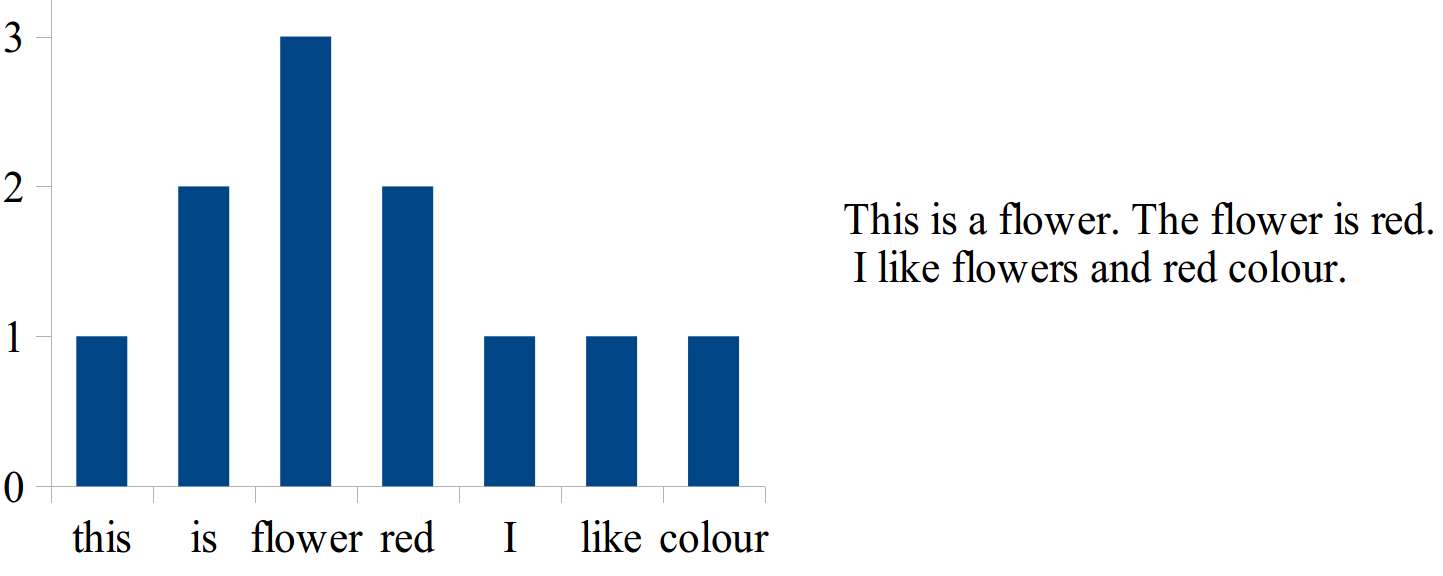
\includegraphics[width=0.7\textwidth]{figs/bow_example}
  \caption{Bag of Words histogram}
  \label{fig:bow_example}
  \end{figure}

  Figure \ref{fig:bow_example} shows a piece of text and its BoW model, with 
articles and punctuation marks left out. To compare different 
documents we need a global dictionary (or codebook), usually constructed by 
taking all unique words from available documents (a training set). If 
a dictionary is of any considerable size the resulting representation of 
especially small documents can be very sparse.

  In natural language processing BoW is used to infer semantic meaning of 
documents. If we could translate an image into a text document we might be able 
to employ similar methods. How do we do that?

  \subsection{From Images to Text Documents}	
The original pipeline consists of the following 
steps: (1) region detection, (2) feature extraction, (3) vector quantization 
and (4) BoW histogram formation as in figure \ref{fig:bow_pipeline}. Tsai 
summarizes the most common methods used recently \cite{tsai2012bag}. 

    \begin{figure}[!ht]
    \centering
    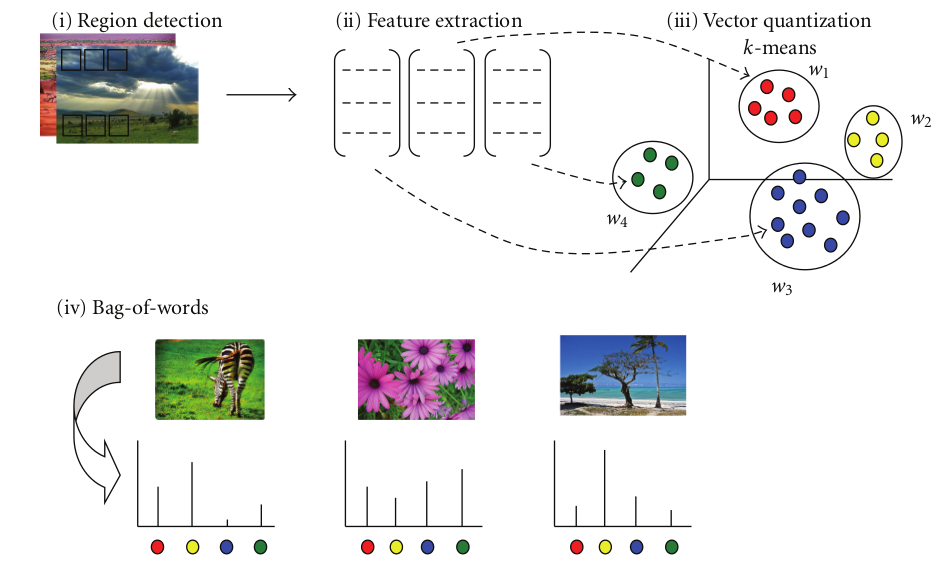
\includegraphics[width=0.75\textwidth]{figs/tsai2012}
    \caption{Bag of Words pipeline. The figure comes from \cite{tsai2012bag}}
    \label{fig:bow_pipeline}
    \end{figure}
	
  \subsubsection{Region Detection}
    Characteristic region detection is the first step in any Bag of Words 
framework. Numerous detection methods have been developed, which makes choosing 
the right one tricky. The most common detectors use a Harris corner detector or 
1\textsuperscript{st} or 2\textsuperscript{nd} image derivatives. A 
Harris-Laplace detector is an example of a Harris-based detector. The Harris 
function is scale adapted and its outcome is subjected to a 
Laplacian-of-Gaussian (LoG) operator, which selects points in scale space. 
2\textsuperscript{nd} image derivatives~---~Hessians can be combined with a LoG 
operator in order to further select points in the Hessian's determinant space.

    A number of more advanced recipes for salient region localization have been 
developed and implemented. These include for example SIFT
and ISS, with the vast majority 
implemented for the 2D domain and only a few generalized to 3D. A comparative 
study of detectors available in the PointCloud Library (PCL) can be found in 
\cite{pcl_keypoint_comparision, 3d_keypoint_eval}. All of the above, called 
sparse feature detectors, resort to selection of maxima in specific state 
spaces. An entirely different scheme is to use a dense feature detector, that 
is to take a uniformly sampled grid of points. Dense detectors are advantageous 
in that they sample slow changing regions in terms of image derivatives. 
Examples of such regions are a clear sky or a calm ocean. It was
showed that dense detectors generally outperform sparse ones 
\cite{tsai2012bag}.
    
  \subsubsection{Feature Extraction}
    Suppose only keypoint's coordinates were given. The smallest affine 
transformation applied to the image would render the keypoints useless. Feature 
extraction is about describing a region in a way that is invariant to affine 
transformations, light intensity changes or color saturation. Achieving all 
these properties simultaneously can be hard but methods that achieve some of 
them do exist. Keypoint description takes form of coordinates in a 
high-dimensional space. One of the most precise and repeatable algorithm is 
SIFT \cite{sift_features}, which is a 3D histogram of gradients structured as a 
128-dimensional vector of floating point values. It is the most often extracted 
descriptor in BoW pipelines. Other methods include various color descriptors, 
binary descriptors such as 512-dimensional GIST. There are 
techniques designed for 3D exclusively. Among them are Persistent Point Feature 
Histogram (PFH) , its faster alternative FPFH 
 and PFHRGB, which takes into account color information, 
all implemented in PCL.
    
  \subsubsection{Vector Quantization}
    Vector quantization comprises of: (1)~codebook construction and 
(2)~descriptor parsing. 

To build a dictionary we have to describe the training set (the previous steps) 
and find patterns in the descriptor space. A codebook can then contain 
centroids (means or medoids) of these patterns. The parsing phase is about 
assigning a descriptor to one of the codebook elements (e.g. 1-nearest 
neighbor matching with a centroid). A parsed descriptor is called a 
\textit{visual word}. Finally, we build a histogram by counting how many times 
each visual word occurred for an image. The result is a fixed-size histogram, 
whose each bin tells us how many times a visual word occurred.

    The KMeans is the single most popular vector quantization algorithm used in 
the BoW pipelines \cite{tsai2012bag}. Developed in 1950's, it is well known and 
easy to implement. KMeans divides all data into a predefined amount of clusters 
and computes their centroids. Many modifications and alternative versions 
emerged \cite{kmeans_jain2010data}. Some of them are: faster than the original 
\emph{approximate KMeans}, \emph{hierarchical KMeans}, which automatically 
chooses the final number of clusters and a \emph{soft KMeans} --- a variation 
that allows fuzzy alignment. Fuzzy alignment means that each point can belong 
to several clusters with different weights (e.g. proportional to the inverse 
square of a distance to a centroid). 
    
    If computational cost is of no concern or if required precision is of the 
utmost priority we can use Gaussian Mixture Model (GMM). It partitions data 
into a set of clusters, finds their means and covariances. In the parsing step 
it computes a probability distribution of a descriptor over all the clusters. 
Fuzzy aligned histogram is built by taking the probability distribution as 
weights. GMM can be thought of as a generalization of the KMeans algorithm. One 
drawback is massive computational cost in comparison with still expensive 
KMeans. Recently, Perronnin \textit{et al} proposed GMM based fisher-kernel 
vector quantization step yielding superior results \cite{fisher1, fisher2}.	
	
    After choosing a vector quantization algorithm a codebook size have to be 
determined. With a standard KMeans implementation the dictionary size defines 
how much information is retained in a BoW histogram. A big trainset containing 
many classes with large intra- and inter-class variance is likely to 
require a huge codebook. On the other hand, too big a dictionary might 
introduce quantization artefacts. We have to bear in mind that the vector 
quantization step is the most time-consuming part of the BoW pipeline. The 
highest computational complexity is associated with the codebook construction 
step and it is $O(n^3)$, where $n$ is the codebook size.		
    
    It is possible to combine several feature extraction algorithms before 
creating the codebook (Early Fusion) or create many codebooks and concatenate 
resulting histograms (Late Fusion). Both schemes are as simple as vector 
concatenation. The Early Fusion concatenates two feature vectors if they have 
been extracted from the same keypoint. The Late Fusion joins histograms that 
are output of separate quantization steps.
	      
\subsection{Problem of Classification}

    To classify means to, given a set of categories, produce a category label 
for a given set of features. Image classification fits this 
description perfectly. The only difficulty lies in complexity of a raw image. 
Suppose we have a $320$ by $240$ three channel color image. This amounts to a 
total of $230400$ dimensions, far too many to feed into any classifier 
directly. Fortunately, a Bag of Words histogram is a compact and discriminative 
intermediate representation that solves this issue. It can be used with any 
classifier. Classifiers can be two-class classifiers (e.g. binary) or 
multi-class classifiers. The latter are often a combination of several binary 
classifiers. The most popular classifiers are: k-Nearest Neighbors, Logistic 
Regression, Softmax Regression, Na\`ive Bayes and Support Vector Machine.

\section{ Datasets}

  Datasets are essential for the following reasons: (1) Supervised learning 
algorithms have ravenous appetite for labeled data. An open database of labeled 
RGBD images would be of great help in evaluation of algorithms. (2) If any 
comparison of algorithms is to be meaningful it should be performed on the same 
data. There is a multitude of RGB datasets available: 
ImageNet\footnote{\url{http://www.image-net.org/}}, 
PascalVoc\footnote{\url{http://pascallin.ecs.soton.ac.uk/challenges/VOC/}}, 
LabelMe\footnote{\url{
http://labelme.csail.mit.edu/Release3.0/browserTools/php/dataset.php}} and 
SUN\footnote{\url{http://groups.csail.mit.edu/vision/SUN/}}, among others. 
Unfortunately, they do not contain any depth information and cannot be used for 
the purpose of object classification based on RGBD data. On the other hand, the 
vast majority of RGBD datasets are focused on tracking or instance-level 
recognition, have insufficient number of examples per category or have too few 
categories. Author managed to find only two datasets suited to his needs. They 
are: the Berkeley 3D Object (B3DO) dataset \cite{B3DO} and a dataset compiled 
by Zhang \emph{et al} at the University of Tokyo\cite{zhangcategory}. The 
latter will be abbreviated Tokyo dataset from now on.

  \subsection{Berkeley 3D Object Dataset}
    \begin{figure}[!ht]
    \centering	
    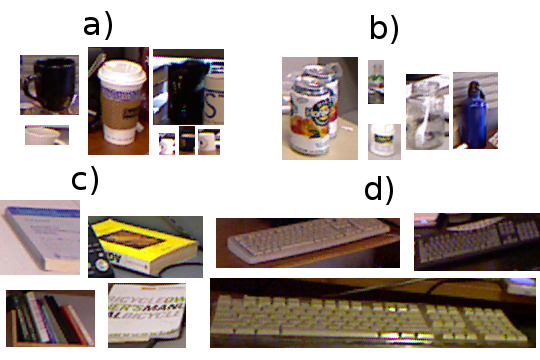
\includegraphics[width=.75\textwidth]{figs/b3do_objects}
    \caption{B3DO objects: a) cups b) bottles c) books d) keyboards}
    \label{fig:b3do_objects}
    \end{figure}    
    
    The Berkeley 3D Object dataset, shown in figure \ref{fig:b3do_objects}, was 
specifically designed for the purpose of object detection and classification. 
It consists of cluttered images in indoor environment, with many labeled and 
random objects per image. The images are often poorly lit and objects are 
partially occluded. There are around 50 classes with more than 20 examples in 
each of them. RGBD data are provided as pairs of color images (8 bit RGB jpeg 
files) and depth maps (16 bit png files). Images are densely labeled --- for 
every pair of images there is an xml file with annotations. Each annotation 
states a category of an object as well as it's bounding box location. Since 
neither image segmentation nor object detection is addressed in this paper we 
had to extract objects from the images before the dataset could be used.

  \subsection{The University of Tokyo Dataset}	
    \begin{figure}[!ht]
    \centering
    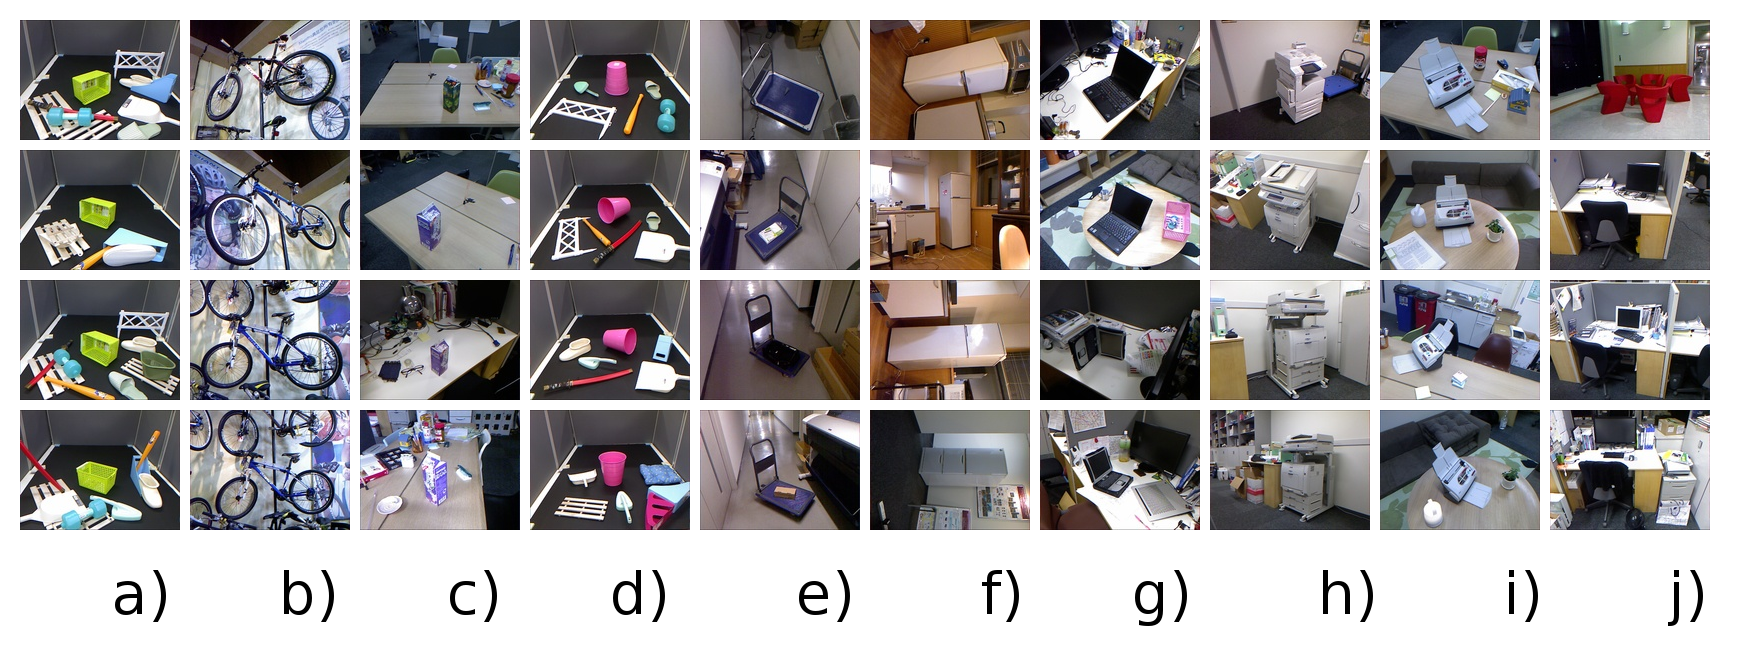
\includegraphics[width=1\textwidth]{figs/tokyo_horizontal}
    \caption{The Tokyo dataset: a) basket b) bicycle c) box d) bucket e) cart 
f) freezer g) notebook h) printer i) scanner j) scene}
    \label{fig:tokyo}
    \end{figure}

    The Tokyo dataset, shown in figure \ref{fig:tokyo}, is comprised of high 
quality images of single labeled objects in different settings, with changing 
viewpoint, object orientation and texture. Additional unlabeled objects can be 
present, however, and should not be taken into account. No bounding boxes are 
given, which renders the classification task similar to the scene 
classification problem. The dataset is presented as color images (8 bit RGB 
jpeg files) and depth maps (csv files with XYZ coordinates of each pixel). This 
dataset is aimed at the task of object classification in casual images.

\section{ Experiments }
  There is a plenty of algorithms suitable for any of the four steps of Bag of 
Words image processing. Most of them have multiple tunable parameters and their 
performance might be interdependent on each other. Comprehensive evaluation is 
inevitable if an optimal combination is to be selected. Considering the 
PointCloud Library\footnote{\url{http://pointclouds.org/}} (PCL) alone yields 
far too many options to test, with 12 keypoint detectors and more than 20 
feature descriptors. A literature review helped to narrow the scope of 
evaluation considerably. All experiments were run on a notebook with Intel Core 
i7 quad core 2.2 GHz CPU, 8 GB of RAM and a nVidia M540 GPU. 

  \subsection{Detectors and descriptors}
    Keypoint detection algorithms were compared with respect to repeatability 
and invariance in \cite{pcl_keypoint_comparision} as well as in terms of object 
retrieval and recognition in \cite{3d_keypoint_eval}. 3D-SIFT and ISS both 
achieve the highest robustness, while the latter appears to be the best choice 
for object retrieval. Dense detector (or uniform sampling) achieves the best 
performance in 2D image classification \cite{tsai2012bag}. Therefore, this 
paper compares SIFT, ISS and Uniform Sampling keypoint detection techniques. 
Additionally, PCL descriptors were evaluated in terms of object retrieval 
performance in \cite{pcl_features}. PFHRGB and SHOTCOLOR delivered the best 
results, while their simpler counterparts (PFH, FPFH, SHOT) were only a little 
worse. USC, which is a global descriptor and thus not suitable for the Bag of 
Words approach, achieved very similar accuracy. The family of PFH descriptors 
is evaluated in this paper.
    
    \begin{table}[!hbtp]
    \centering
      \caption{Highest accuracy obtained with FPFH, PFH and PFHRGB descriptors 
on the B3DO dataset}
      \label{tab:desc_b3do}
     \begin{tabular}{*4c}
     \toprule
       Detector & ISS3D & SIFT & Uniform Sampling  \\ 
       Descriptor & \multicolumn{3}{c}{Accuracy {[\%]}} \\
     \midrule
       FPFH & 65.22 &  56.52 & 56.07  \\ 
       PFH & 59.32 &  54.83 & 59.50 \\
       PFHRGB & 63.35 & 52.34 & 53.27 \\
       
   \bottomrule
    \end{tabular}
    \end{table}

    The best results of each detector/descriptor combination on the B3DO 
dataset are shown in table \ref{tab:desc_b3do}. ISS consistently proved to be 
the most successful detection algorithm in this setting. SIFT and Uniform 
Sampling scored similar accuracy but the latter is significantly faster. SIFT 
is in fact the slowest of the three. As for the descriptors, FPFH delivered the 
best performance, even though it is an approximate and theoretically the least 
precise algorithm. It is also the fastest of the three. The combination of ISS 
and FPFH delivers outstanding results at the lowest computational cost. It 
allows near real time point-cloud processing and classification. PFHRGB and 
SIFT are several times slower.
      
  \subsection{Codebook}
    KMeans is used in almost every implementation of the Bag of Words image 
processing pipeline \cite{tsai2012bag}. The number of visual words can have a 
significant impact on the final results. A number of tests were run to discover 
an optimal codebook size for the current setting.

    \begin{figure}[!ht]
    \centering	
    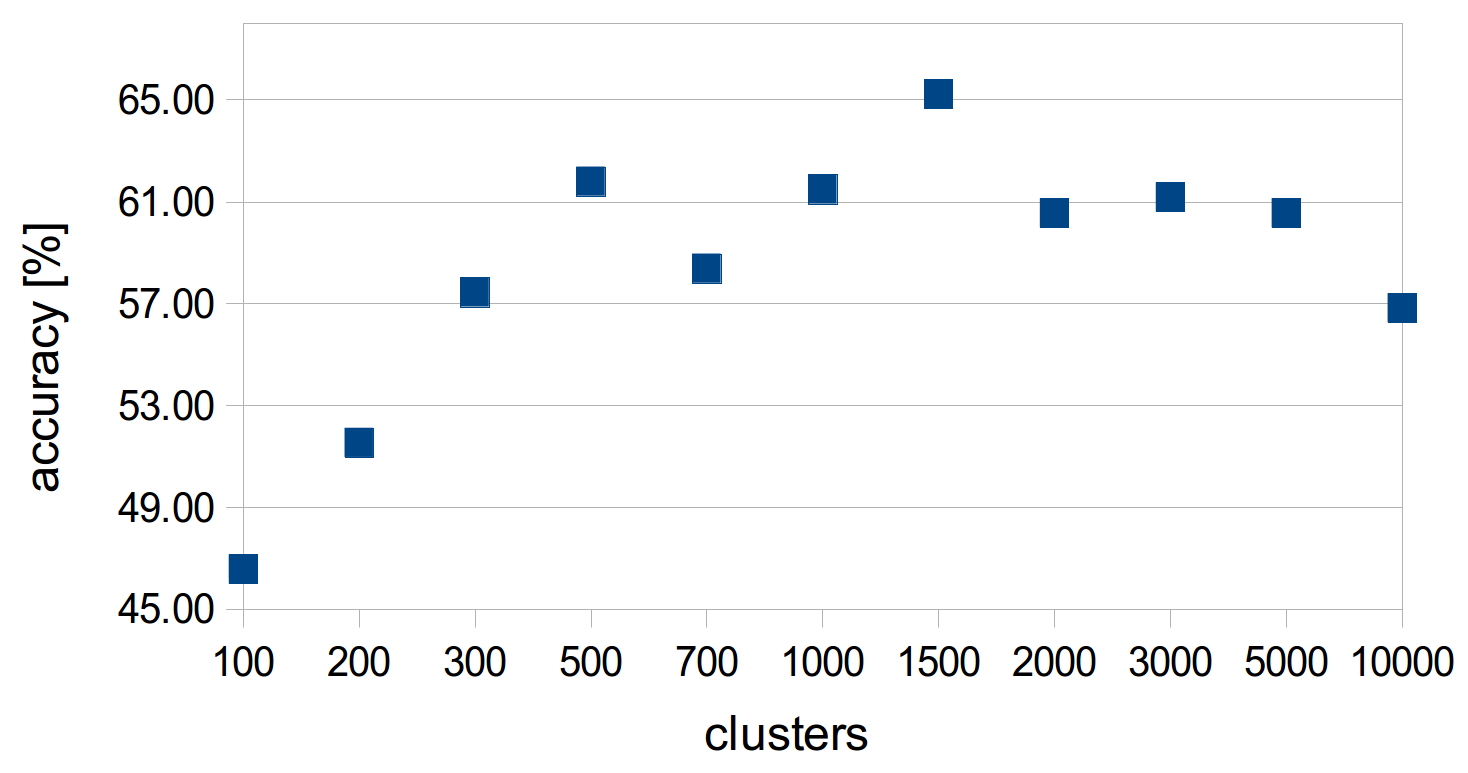
\includegraphics[width=.75\textwidth]{figs/clustering_centroids_b3do}
    \caption{Influence of dictionary size on the overall accuracy. B3DO dataset 
with ISS keypoint detector and FPFH feature descriptor}
    \label{fig:cluster_b3do}
    \end{figure}

    The results from figure \ref{fig:cluster_b3do} partially confirm Csurka's 
findings. The performance raises with the increasing number of centroids up to 
the point of 1500 centroids and 65.22\%. The discrepancies might be caused by 
the following factors: (1) ISS detector finds too many or irrelevant points, 
thus introducing noise or (2) The FPFH descriptor has too few dimensions (33) 
to be divided into more than 1500 regions in a meaningful way. 


  \subsection{B3DO}
    Extracting objects from the B3DO datasets yielded far too many and 
unbalanced categories. The number of objects in each category varies from 1 
(tape) to 299 (table). 8 categories were picked at random with a restriction 
that there should be at least 50 object instances in a category. Then, the 
objects were split into train and test set with a proportion of 1:1, which were 
used for estimation and evaluation respectively.

    The highest accuracy achieved for this dataset is 65.22\%. Table 
\ref{tab:b3do_conf_matrix} contains a confusion matrix, number of examples per 
category and accuracy. The confusion matrix depicts classification errors. Let 
$m_{i, j}$ be an element of the confusion matrix at the $i^{th}$ row and 
$j^{th}$ column. It shows how many elements from the $i^{th}$ category was 
assigned to the $j^{th}$ category. A high value of $m_{i, j}$ such that $i \neq 
j$ indicates that the classifier cannot distinguish those two classes.

    \begin{table}[!ht]
    \centering
    \caption{Results on the B3DO dataset with ISS keypoint detector, FPFH 
features and a dictionary of 1500 words; \textbf{Average accuracy: 65.22\%}}
    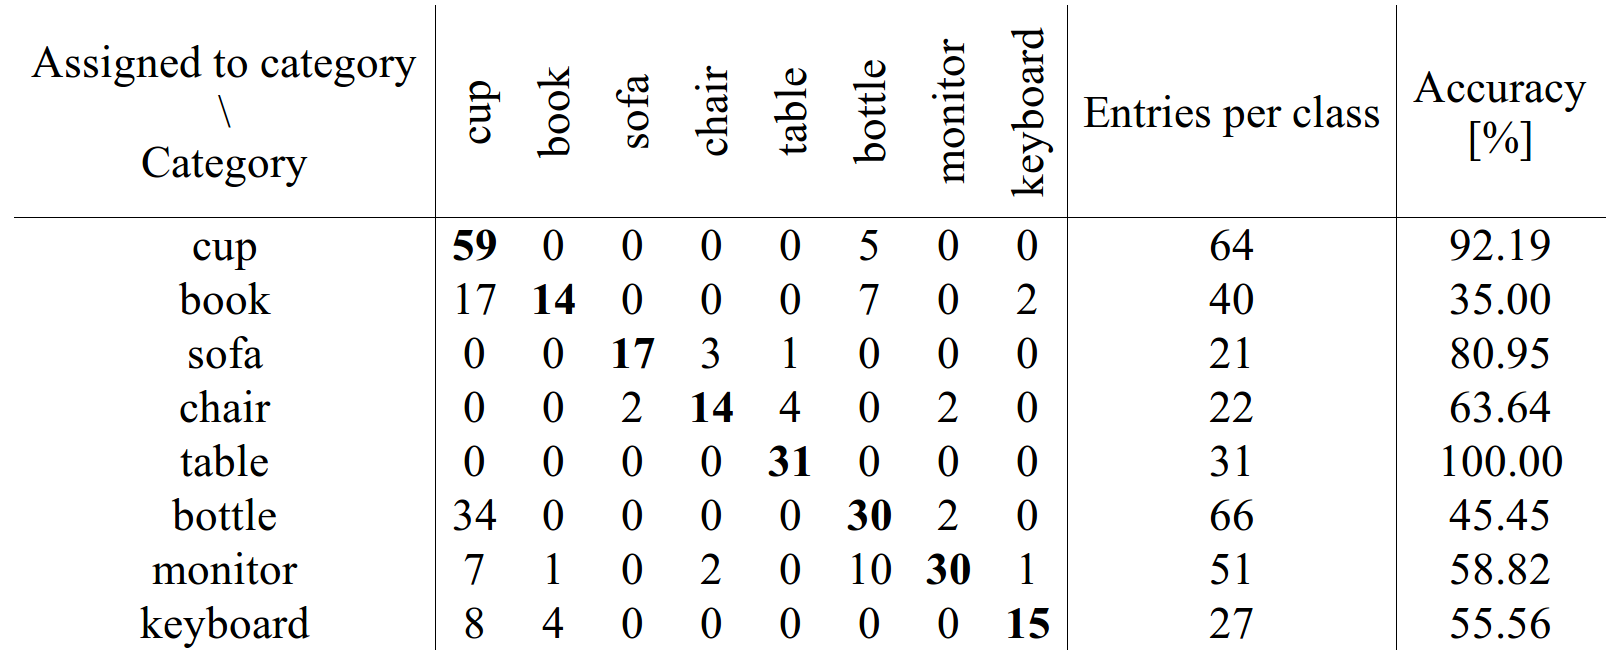
\includegraphics[width=0.9\textwidth]{figs/b3do_conf_matrix}	
    \label{tab:b3do_conf_matrix}
    \end{table}   

    More than half of the bottles were assigned to the cup category and 
keyboards were often mistook for books. These two error types are easily 
explained by a high degree of similarity of objects (bottles and cups are 
usually round and tall, books and keyboards are flat and rectangular) 
Surprisingly, however, objects from half of the categories were frequently 
marked as cups. Some of these misclassification errors might be caused by very 
poor quality of images. Many of them are occluded poorly lit low resolution 
images.	

  \subsection{Tokyo}
    \begin{table}[!ht]
    \centering
    \caption{Results on the Tokyo dataset with ISS keypoint detector, PFH 
features and a dictionary of 3000 words; \textbf{Average accuracy: 62.30\%}}
    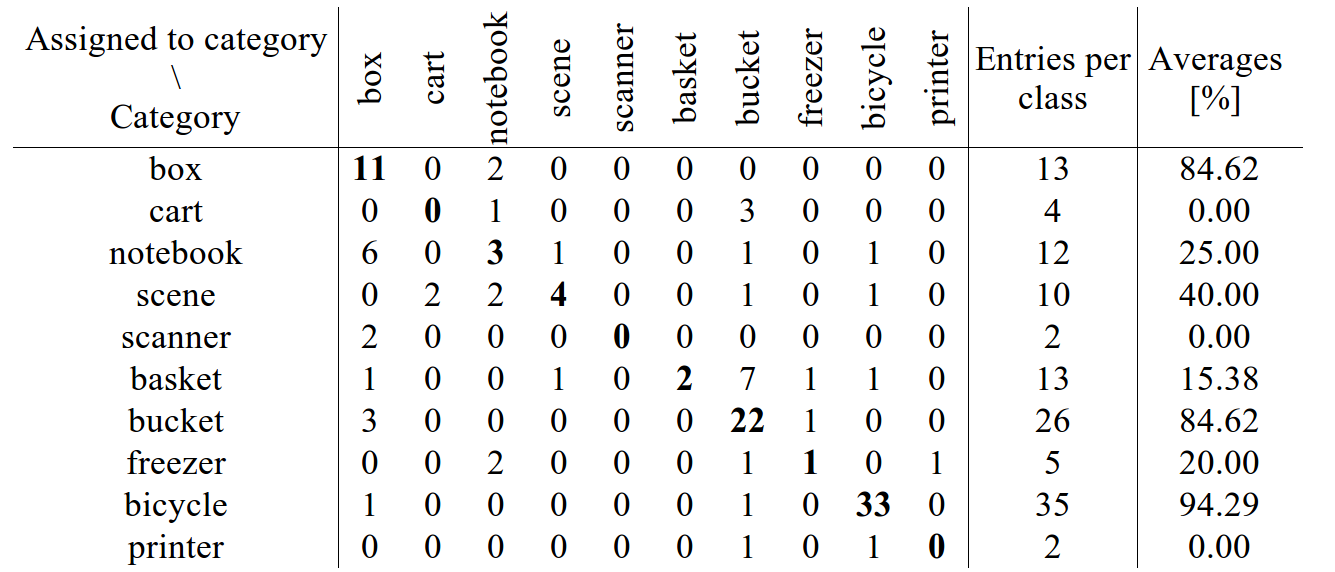
\includegraphics[width=1\textwidth]{figs/tokyo_conf_matrix}	
    \label{tab:tokyo_conf_matrix}
    \end{table}

    Everyone of the 343 images from the Tokyo dataset were used. Data were 
split into test and train set in proportions 1:2 in order to provide more 
training examples due to very limited numbers of objects in some classes. Even 
tough the overall accuracy achieved on the Tokyo dataset is similar in value to 
that of the B3DO's, the structure of the result is very different as shown in 
table \ref{tab:tokyo_conf_matrix}. It is clearly visible that there is a strong 
correlation between a per class accuracy and the number of entries in this 
class. The highest performance in the bicycle category is coupled with the 
largest number of entries. On the other end of the scale there are the printer, 
scanner and cart categories with 2, 2 and 4 entries respectively and 0\% 
classification accuracy. On top of that, the differences between some classes 
are marginal. The majority of carts and baskets were put into the bucket 
category. It does not surprise, for they are simply akin as can be seen in 
figure \ref{fig:tokyo}.

\section{ Conclusion }

  In this paper the issue of three dimensional point cloud classification with 
a bag of words-based approach was tackled. Two scientific databases suitable 
for the task of point cloud classification were identified and adapted for the 
purpose of this work. Presence of such datasets is vital --- they act as 
benchmarks and allow objective comparison of different solutions of the 
problem. The following problems emerged: (1)~Point cloud processing is 
computationally expensive and inefficient. Due to the lack of structure in 
point clouds (\textit{i.e.} no predefined spatial relationships between points) 
additional calculations have to be performed (\textit{e.g.} finding nearest 
neighbors requires at least several distance computations). (2)~There are very 
few and small databases available. Machine learning algorithms have ravenous 
appetite for labeled data. As the newest findings in the state-of-the-art 2D 
object classification suggest, an order of tens of thousands of samples is a 
prerequisite for any satisfactory results. This work had to make do with less 
than 300 objects in the train sets. (3)~There is very little interest in the 
scientific community for this particular task. The majority of research is 
conducted on retrieval of CAD-like objects from mesh databases.
  
  The achieved results the B3DO and Tokyo datasets are respectively $5.21$ and 
$6.23$ times higher than random rates ($12.5\%$ and $10\%$). This shows that 
classification of point clouds is feasible and can be performed in what is 
close to real time on a mainstream notebook. The accuracy can be further 
enhanced by generalizing 2D algorithms to the 3D domain, while the 
computational time can be reduced by using a GPU for the most computationally 
expensive parts of the Bag of Words framework. In conclusion, the depth data 
does not account for a straightforward improvement in classification accuracy. 
In fact, it is easier to obtain better results on 2D RGB images, because the 
best algorithms are not converted to the 3D domain and there is substantially 
more data available for the 2D. 

\bibliography{kkr13}
\end{document}



